% -------------------------
% Raport koncowy projektu: System monitorowania obecnosci i upadkow czlowieka
% Kompiluje sie kazdym silnikiem: pdflatex, xelatex, lualatex, tectonic.
% (Na Overleaf dziala niezaleznie od ustawienia "Compiler".)
% Strona tytulowa = oficjalny druk RAu6 (osobny plik, doklejany z przodu przy scalaniu PDF).
% -------------------------
\documentclass[11pt,a4paper]{article}

\usepackage{iftex}
\ifPDFTeX
  \usepackage[T1]{fontenc}
  \usepackage[utf8]{inputenc}
  \usepackage{lmodern}
\else
  \usepackage{fontspec}
\fi
\usepackage[polish]{babel}
\usepackage[a4paper,margin=2.5cm]{geometry}
\usepackage{graphicx}
\graphicspath{{img/}}
\usepackage{float}
\usepackage{array}
\usepackage{tabularx}
\usepackage{booktabs}
\usepackage{enumitem}
\usepackage{textcomp}
\usepackage{caption}
\usepackage{fancyhdr}
\usepackage{tikz}
\usetikzlibrary{positioning,arrows.meta}
\usepackage[hidelinks]{hyperref}

\setlist{itemsep=2pt,topsep=3pt,parsep=0pt}
\captionsetup{font=small,labelfont=bf,skip=6pt}
\renewcommand{\arraystretch}{1.3}
\setlength{\tabcolsep}{10pt}
\newcolumntype{L}{>{\raggedright\arraybackslash}X}
\newcolumntype{P}[1]{>{\raggedright\arraybackslash}p{#1}}

% delikatny naglowek/stopka -- bez ozdobnikow
\pagestyle{fancy}
\fancyhf{}
\fancyhead[L]{\footnotesize System monitorowania obecno\'sci cz\l owieka}
\fancyhead[R]{\footnotesize Raport ko\'ncowy}
\fancyfoot[C]{\footnotesize \thepage}
\renewcommand{\headrulewidth}{0.4pt}
\renewcommand{\footrulewidth}{0pt}

% numery sekcji z kropka (jak w Analizie projektu)
\renewcommand{\thesection}{\arabic{section}.}
\renewcommand{\thesubsection}{\arabic{section}.\arabic{subsection}.}

\begin{document}

\begin{center}
  {\Large\bfseries System monitorowania obecno\'sci cz\l owieka}\\[0.3em]
  {\large Raport ko\'ncowy projektu}
\end{center}
\vspace{1.5em}

{\setlength{\parskip}{0pt}\tableofcontents}
\newpage

\begin{abstract}
\noindent
Celem projektu by\l o zaprojektowanie i~zbudowanie dzia\l aj\k acego prototypu
bezkontaktowego systemu monitorowania obecno\'sci cz\l owieka, ukierunkowanego na
bezpiecze\'nstwo os\'ob starszych mieszkaj\k acych samotnie. System rozpoznaje cztery
klasy zdarze\'n: obecno\'s\'c, upadek, po\.zar oraz d\l ugotrwa\l y
bezruch. Rozpoznanie opiera si\k e na danych z~radaru fal milimetrowych 60~GHz,
bez rejestracji obrazu. Dane s\k a odczytywane po magistrali I\textsuperscript{2}C
przez mikrokontroler ESP32-C6, kt\'ory klasyfikuje sytuacj\k e lokalnie
(\emph{edge computing}) i~publikuje status w~formacie JSON do brokera MQTT.
Przegl\k adarkowy panel opiekuna subskrybuje brokera przez WebSocket i~pokazuje
stan pomieszcze\'n w~czasie rzeczywistym, wraz z~alarmem d\'zwi\k ekowym i~rozr\'o\.znieniem
stanu ,,pusty pok\'oj'' od ,,utrata \l \k aczno\'sci''. Efektem prac jest kompletny,
dzia\l aj\k acy przep\l yw \emph{end-to-end}: czujnik $\rightarrow$ firmware $\rightarrow$
broker $\rightarrow$ panel. Konfiguracja Wi-Fi i~adresu brokera odbywa si\k e
z~telefonu przez \emph{captive portal}, bez zaszywania danych w~kodzie.
\end{abstract}

% ===========================================================================
\section{Wprowadzenie}

Starzenie si\k e spo\l ecze\'nstwa czyni bezpiecze\'nstwo samotnie mieszkaj\k acych
senior\'ow problemem o~rosn\k acej skali. Upadek pozostawiony bez pomocy przez wiele
godzin jest jedn\k a z~najcz\k estszych dr\'og do utraty samodzielno\'sci, a~w~skrajnych
przypadkach zagra\.za \.zyciu. Istniej\k ace rozwi\k azania (kamery, opaski
i~przyciski SOS) maj\k a istotne wady: naruszaj\k a prywatno\'s\'c, wymagaj\k a noszenia
i~\l adowania albo s\k a bezu\.zyteczne, gdy poszkodowany jest nieprzytomny.

Celem projektu by\l o opracowanie bezobs\l ugowego, nieinwazyjnego systemu, kt\'ory
wykrywa obecno\'s\'c i~zdarzenia zagra\.zaj\k ace zdrowiu bez udzia\l u u\.zytkownika
i~bez rejestracji obrazu. Zakres prac obj\k a\l: (1)~analiz\k e technologii detekcji,
(2)~rozpoznanie rynku i~dob\'or komponent\'ow, (3)~projekt architektury sprz\k etowej
i~programowej, (4)~implementacj\k e firmware realizuj\k acego lokaln\k a klasyfikacj\k e
zdarze\'n oraz (5)~budow\k e panelu opiekuna prezentuj\k acego status w~czasie
rzeczywistym.

Przyj\k eto, \.ze jeden czujnik radarowy pod sufitem wystarczy do rozpoznania
obecno\'sci, oddechu i~upadku w~pomieszczeniu, bez rejestracji obrazu i~bez
urz\k adze\'n noszonych przez u\.zytkownika.

% ===========================================================================
\section{Kontekst i~analiza rynku}

\subsection{Skala problemu}

W~Polsce mieszka ok.\ 10~mln os\'ob w~wieku 60+ (oko\l o 25\%\ spo\l ecze\'nstwa), a~coraz
wi\k eksza ich cz\k e\'s\'c \.zyje samotnie. Upadki s\k a dominuj\k ac\k a przyczyn\k a
hospitalizacji w~tej grupie wiekowej. Wed\l ug danych NCOA/CDC (USA) senior trafia
na izb\k e przyj\k e\'c po upadku \'srednio co 11~sekund, a~jedna na cztery starsze
osoby upada w~ci\k agu roku. Kluczowy jest czas reakcji. Pomoc udzielona szybko
po upadku decyduje o~dalszej samodzielno\'sci.

\vspace{2pt}
{\small\itshape \'Zr\'od\l a: GUS, ,,Sytuacja os\'ob starszych w~Polsce 2024'',
NCOA/CDC (USA).\par}

\subsection{Luka rynkowa}

Trzy najpopularniejsze podej\'scia do monitorowania senior\'ow maj\k a ograniczenia,
kt\'ore dyskwalifikuj\k a je w~typowym \'srodowisku domowym
(tabela~\ref{tab:luka}).

\begin{table}[htbp]
\centering
\caption{Ograniczenia istniej\k acych rozwi\k aza\'n.}
\label{tab:luka}
\begin{tabularx}{\linewidth}{@{}P{0.30\linewidth} L@{}}
\toprule
\textbf{Rozwi\k azanie} & \textbf{G\l \'owne ograniczenie}\\
\midrule
Kamera & Narusza prywatno\'s\'c (\l azienka, sypialnia), nie dzia\l a w~ciemno\'sci.\\
Opaska / smartwatch & Trzeba pami\k eta\'c o~noszeniu i~regularnym \l adowaniu.\\
Przycisk SOS & Bezu\.zyteczny, gdy osoba jest nieprzytomna lub unieruchomiona po upadku.\\
\bottomrule
\end{tabularx}
\end{table}

Odbiorcami rozwi\k azania s\k a domy opieki, opieka domowa, szpitale oraz rodziny
senior\'ow, co otwiera mo\.zliwo\'s\'c u\.zycia modelu \l \k acz\k acego sprzeda\.z lub wynajem
sprz\k etu (B2C) z~licencjami plac\'owek i~panelem zbiorczym (B2B).

% ===========================================================================
\section{Analiza techniczna}

\subsection{Metoda detekcji}

Rozwa\.zono trzy technologie bezkontaktowej detekcji obecno\'sci
(tabela~\ref{tab:metoda}). Radar fal milimetrowych jako jedyny zapewnia
wystarczaj\k ac\k a dok\l adno\'s\'c bez rejestracji obrazu.

\begin{table}[htbp]
\centering
\caption{Por\'ownanie metod detekcji.}
\label{tab:metoda}
\begin{tabularx}{\linewidth}{@{}P{0.26\linewidth} L@{}}
\toprule
\textbf{Technologia} & \textbf{Ocena}\\
\midrule
PIR (pasywna podczerwie\'n) & Najta\'nsza. Wykrywa tylko du\.ze zmiany temperatury, nie widzi os\'ob \'spi\k acych i~nieruchomych. \emph{Odrzucona.}\\
Kamera + analiza obrazu & Bardzo dok\l adna. Narusza prywatno\'s\'c i~wymaga du\.zej mocy obliczeniowej. \emph{Odrzucona.}\\
Radar fal milimetrowych & Przenika odzie\.z i~cienkie przeszkody, nie rejestruje obrazu, wykrywa mikroruchy (oddech). \textbf{Wybrana.}\\
\bottomrule
\end{tabularx}
\end{table}

\subsection{Sensor radarowy}

Por\'ownano trzy modu\l y radarowe dost\k epne na rynku (tabela~\ref{tab:sensor}).
Decyduj\k aca by\l a zdolno\'s\'c detekcji mikroruch\'ow (ruch klatki piersiowej -
oddech), krytyczna dla funkcji medycznych.

\begin{table}[htbp]
\centering
\caption{Por\'ownanie modu\l\'ow radarowych.}
\label{tab:sensor}
\begin{tabularx}{\linewidth}{@{}P{0.19\linewidth} P{0.09\linewidth} L@{}}
\toprule
\textbf{Modu\l} & \textbf{Pasmo} & \textbf{Detekcja mikroruch\'ow i~decyzja}\\
\midrule
RCWL-0516 & 3~GHz & Bardzo s\l aba (tylko du\.zy ruch). \emph{Odrzucony} - zbyt prosty, brak danych do analizy.\\
HLK-LD2410 & 24~GHz & \'Srednia, ma\l a precyzja. \emph{Odrzucony} - za s\l aby do funkcji medycznych.\\
Acconeer A121 & 60~GHz & Bardzo dobra (ruch klatki piersiowej). \textbf{Wybrany} - najwy\.zsza rozdzielczo\'s\'c, wykrywa mikroruch i~makroruch.\\
\bottomrule
\end{tabularx}
\end{table}

\subsection{Wariant implementacji radaru A121}

Sam czujnik A121 wymaga\l by lutowania BGA i~projektowania w\l asnych anten, dlatego
szukano gotowego modu\l u (tabela~\ref{tab:wariant}).

Gotowy modu\l\ eliminuje projektowanie skomplikowanych obwod\'ow i~lutowanie BGA.
Zintegrowane translatory napi\k e\'c pozwalaj\k a pod\l \k aczy\'c modu\l\ bezpo\'srednio
do pinu 5~V mikrokontrolera. Zachowana zostaje precyzja 60~GHz przy pomini\k eciu
koszt\'ow oficjalnych zestaw\'ow ewaluacyjnych.

\begin{table}[H]
\centering
\caption{Warianty implementacji radaru Acconeer~A121.}
\label{tab:wariant}
\begin{tabularx}{\linewidth}{@{}P{0.30\linewidth} L@{}}
\toprule
\textbf{Wariant} & \textbf{Decyzja i~uzasadnienie}\\
\midrule
Acconeer A121 (go\l y czujnik) & \emph{Odrzucony} - lutowanie BGA i~w\l asne anteny.\\
SparkFun XM125 & \emph{Odrzucony} - wysoka cena, brak dost\k epno\'sci.\\
Acconeer XE125 (zestaw ewaluacyjny) & \emph{Odrzucony} - bardzo wysoka cena, rozbudowana platforma testowa.\\
Modu\l\ Acconeer XM125 & \emph{Odrzucony} - rozwi\k azuje tor radiowy, ale wymaga w\l asnej p\l yty bazowej i~zasilania.\\
Waveshare A121 mmWave & \textbf{Wybrany} - zintegrowany STM32, antena i~stabilizatory napi\k ecia. Eliminuje lutowanie BGA i~upraszcza zasilanie.\\
\bottomrule
\end{tabularx}
\end{table}

\subsection{Mikrokontroler}

Por\'ownano serie uk\l ad\'ow ESP32 (tabela~\ref{tab:mcu}). Wybrano ESP32-C6 -
jedyn\k a seri\k e \l \k acz\k ac\k a energooszcz\k edno\'s\'c z~pe\l nym zestawem protoko\l\'ow
bezprzewodowych IoT.

\begin{table}[htbp]
\centering
\caption{Por\'ownanie serii ESP32.}
\label{tab:mcu}
\begin{tabularx}{\linewidth}{@{}P{0.17\linewidth} L P{0.14\linewidth}@{}}
\toprule
\textbf{Seria} & \textbf{Rdze\'n / \l \k aczno\'s\'c} & \textbf{Decyzja}\\
\midrule
P-Series (P4) & RISC-V 2$\times$400~MHz, bez radia & \emph{Odrzucona}\\
S-Series (S3) & Xtensa 2$\times$240~MHz, Wi-Fi~4 + BLE~5.0 & \emph{Odrzucona}\\
H-Series (H2) & RISC-V 96~MHz, 802.15.4 + BLE~5.3 & \emph{Odrzucona}\\
C-Series (C6) & RISC-V 160~MHz + rdze\'n LP, Wi-Fi~6 + BLE~5.3 + Zigbee/Thread & \textbf{Wybrana}\\
\bottomrule
\end{tabularx}
\end{table}

Wi-Fi~6 (802.11ax) zapewnia stabilniejsz\k a komunikacj\k e i~lepsze zarz\k adzanie
energi\k a. Koprocesor Low-Power (LP) nas\l uchuje przerwa\'n z~radaru, gdy g\l \'owny
rdze\'n \'spi, minimalizuj\k ac pob\'or pr\k adu. Obs\l uga Zigbee/Thread otwiera
przysz\l \k a integracj\k e z~automatyk\k a budynkow\k a.

\subsection{Aktuatory, sygnalizacja, wej\'scia i~zasilanie}

Warstwa lokalnej interakcji jest minimalna: buzzer wyzwala alarm d\'zwi\k ekowy,
dioda LED pe\l ni rol\k e wska\'znika statusu, a~przycisk s\l u\.zy do r\k ecznego
kasowania alarmu i~resetu konfiguracji. ESP32-C6 wykorzystuje sze\'s\'c pin\'ow
GPIO: magistrala I\textsuperscript{2}C do radaru (SDA, SCL), linia \texttt{MCU\_INT}
radaru oraz buzzer, dioda i~przycisk. Pin \texttt{WAKE\_UP} radaru jest
podci\k agni\k ety na sta\l e do 3,3~V, wi\k ec nie zajmuje GPIO. Zasilanie 5~V
i~wsp\'oln\k a mas\k e rozprowadzono osobno.

Zasilanie: zewn\k etrzne 5~V z~portu USB pod\l \k aczone do modu\l u ESP32-C6-DevKit.
Napi\k ecie 5~V jest wyprowadzone z~pin\'ow ESP32 do modu\l u radaru. Oba modu\l y
wykorzystuj\k a w\l asne, wbudowane stabilizatory LDO, dzi\k eki czemu g\l \'owny schemat
zasilania jest maksymalnie uproszczony.

\subsection{Schemat ideowy i~prototyp}

Warstw\k e sprz\k etow\k a zaprojektowano w~KiCad. Schemat ideowy (rys.~\ref{fig:sch})
obejmuje modu\l\ ESP32-C6-DevKit (U1), modu\l\ radaru Waveshare~A121 (U2), diod\k e
sygnalizacyjn\k a z~rezystorem 330~$\Omega$, przycisk oraz buzzer sterowany
tranzystorem 2N2222 z~rezystorem bazowym 1~k$\Omega$. Przypisanie wyprowadze\'n
w~firmware: \texttt{SDA}~=~GPIO2, \texttt{SCL}~=~GPIO11, \texttt{MCU\_INT}~=~GPIO10,
dioda~=~GPIO18, przycisk~=~GPIO9, buzzer~=~GPIO3. Pin \texttt{WAKE\_UP} radaru jest
zwarty na sta\l e do 3,3~V. Zaprojektowano te\.z wst\k epne rozmieszczenie element\'ow na dedykowanej
p\l ytce PCB (rys.~\ref{fig:pcb}) pod docelow\k a, zminiaturyzowan\k a wersj\k e
urz\k adzenia. Zmontowany prototyp na p\l ytce uniwersalnej pokazano na
rys.~\ref{fig:proto}.

\begin{figure}[H]
\centering
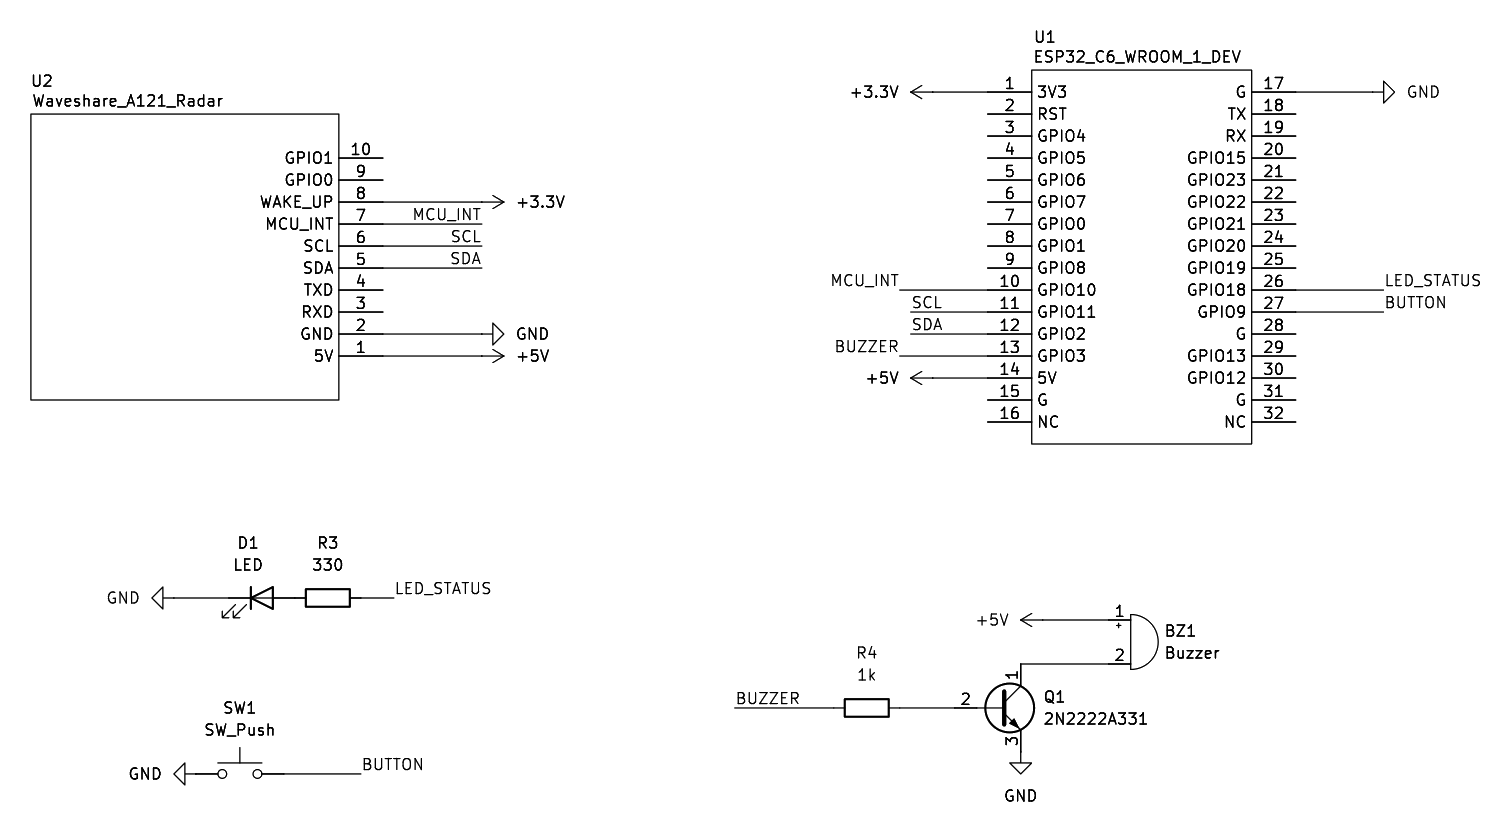
\includegraphics[width=\linewidth]{schemat_ideowy.png}
\caption{Schemat ideowy uk\l adu (KiCad). Wersja podstawowa. W~prototypie diod\k e
sygnalizacyjn\k a uzupe\l niono dodatkow\k a diod\k a RGB wbudowan\k a w~modu\l\ ESP32-C6.}
\label{fig:sch}
\end{figure}

\emph{Uwaga wdro\.zeniowa:} krytyczny jest pin \texttt{WAKE\_UP} podci\k agni\k ety do
3,3~V. Bez niego STM32 na module pozostaje w~trybie Deep~Sleep i~odpowiada po
I\textsuperscript{2}C samymi zerami, co \l atwo pomyli\'c z~b\l \k edem okablowania.

\begin{figure}[H]
\centering
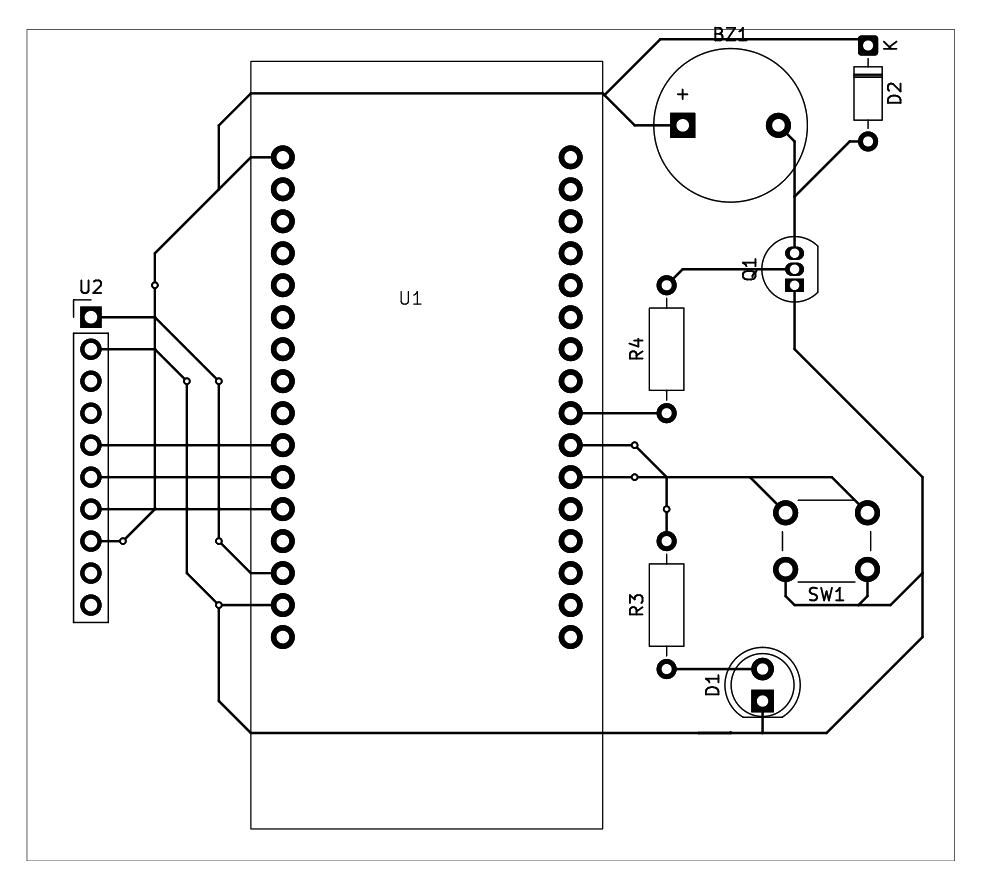
\includegraphics[width=0.58\linewidth]{pcb_layout.png}
\caption{Rozmieszczenie element\'ow i~po\l \k aczenia na dedykowanej p\l ytce PCB.}
\label{fig:pcb}
\end{figure}

\begin{figure}[H]
\centering
\IfFileExists{img/urzadzenie.jpg}
  {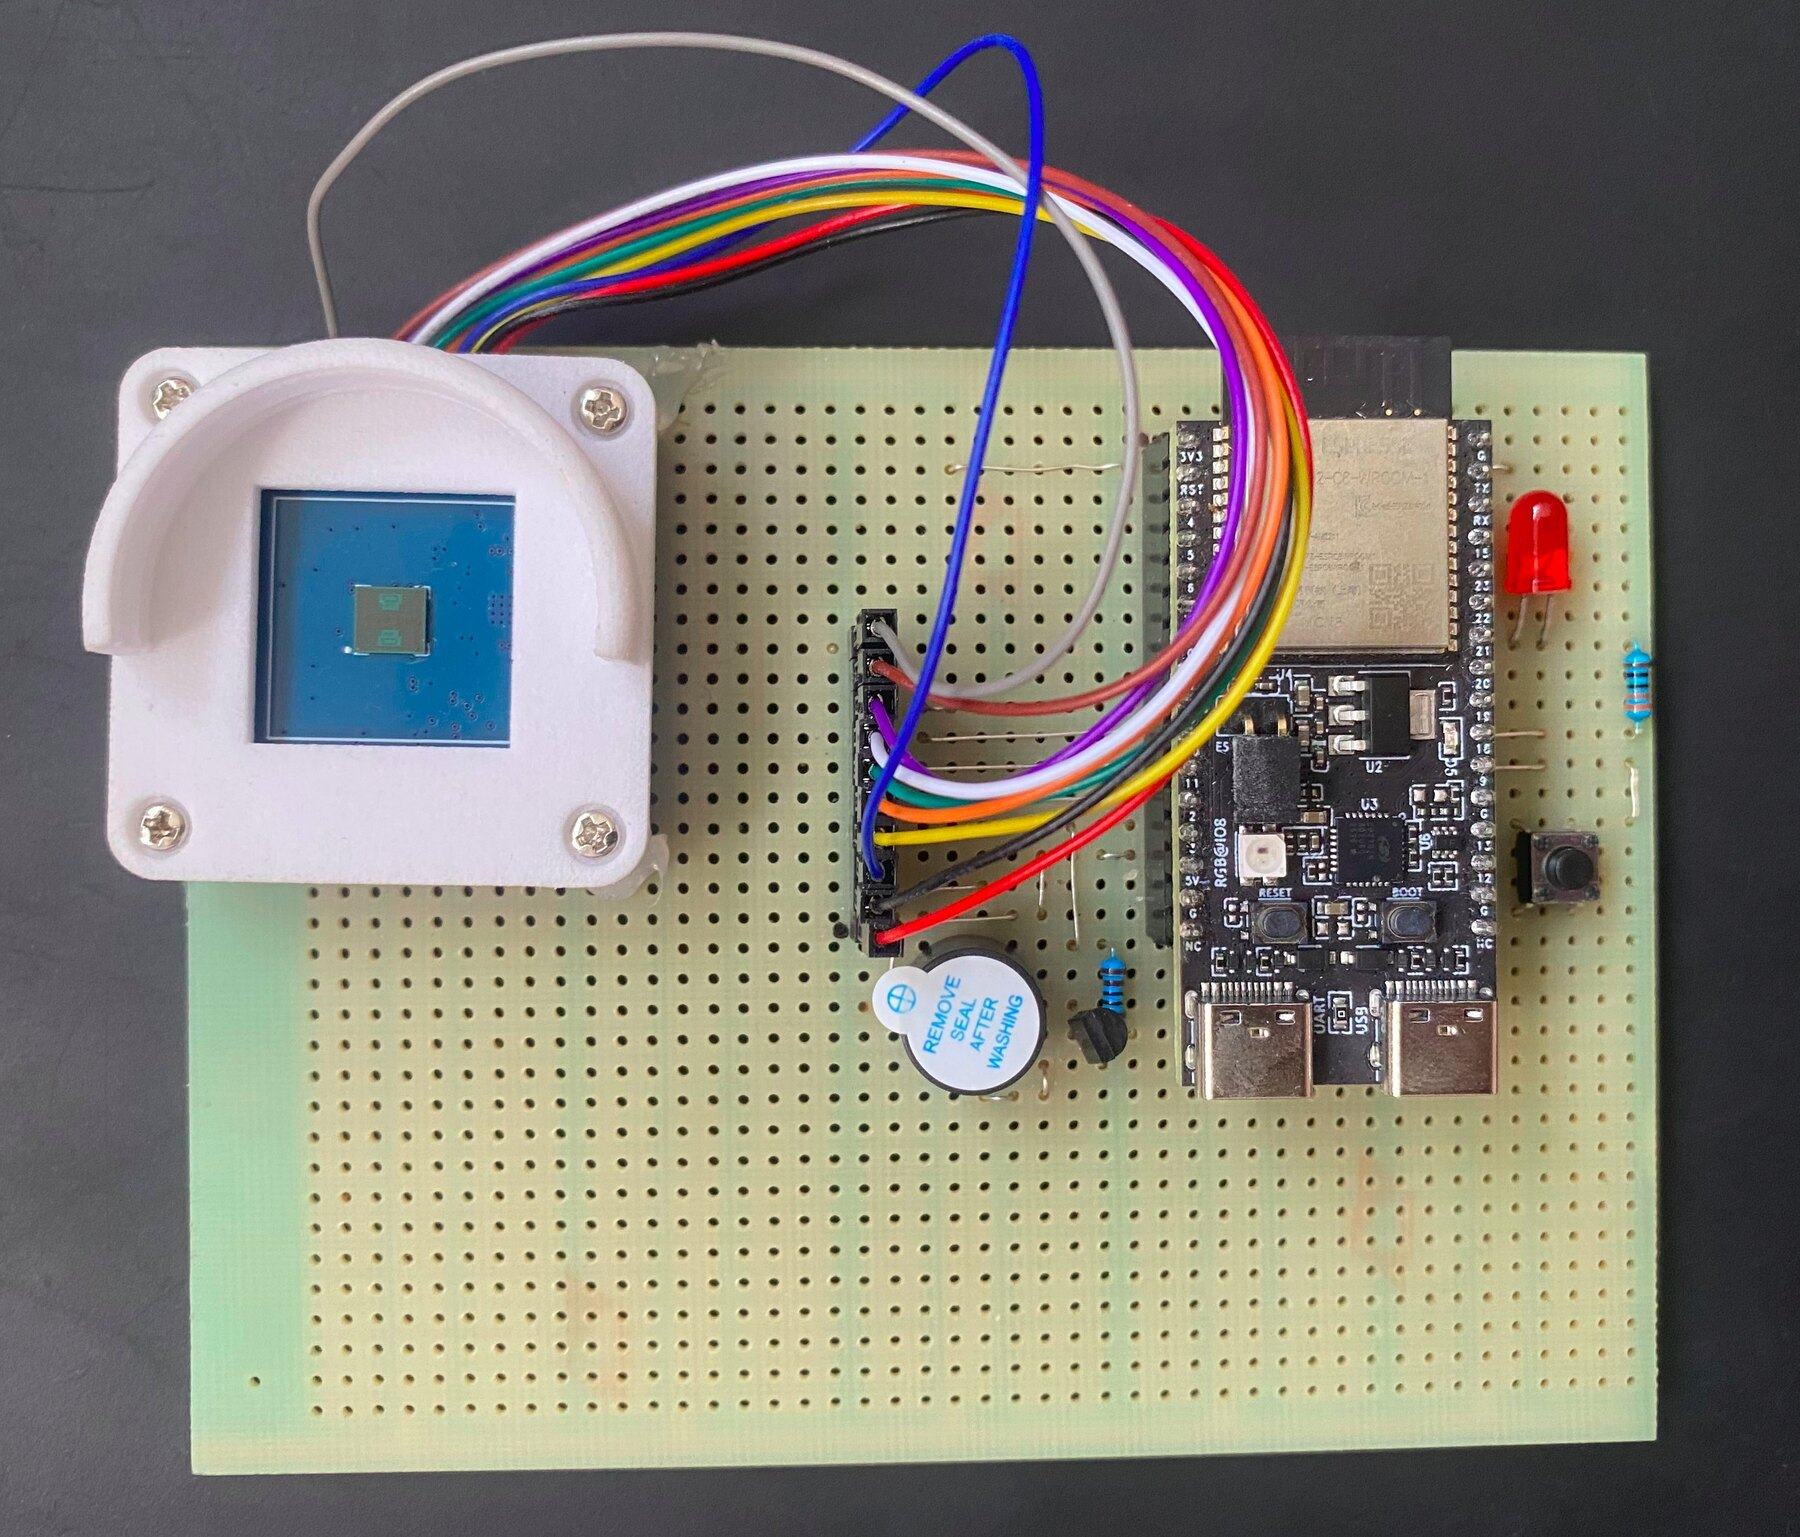
\includegraphics[width=0.68\linewidth]{urzadzenie.jpg}}
  {\fbox{\parbox[c][42mm][c]{0.68\linewidth}{\centering\itshape\small
   Miejsce na zdj\k ecie zmontowanego prototypu\\ (wgra\'c plik \texttt{img/urzadzenie.jpg})}}}
\caption{Zmontowany prototyp urz\k adzenia.}
\label{fig:proto}
\end{figure}

\subsection{Szacunkowy koszt prototypu}

Koszt budowy jednego egzemplarza zebrano w~tabeli~\ref{tab:koszt}. Ceny s\k a
orientacyjne, z~detalicznej sprzeda\.zy modu\l\'ow.

\begin{table}[H]
\centering
\caption{Szacunkowy koszt prototypu.}
\label{tab:koszt}
\begin{tabularx}{\linewidth}{@{}L P{0.22\linewidth}@{}}
\toprule
\textbf{Element} & \textbf{Koszt}\\
\midrule
Modu\l\ radaru Waveshare~A121 (A121 + STM32) & 100~z\l\\
ESP32-C6-DevKit & 36~z\l\\
Buzzer, dioda RGB, przycisk, rezystory & ok.\ 10~z\l\\
P\l ytka uniwersalna, przewody, drobne elementy & ok.\ 10~z\l\\
\midrule
\textbf{Razem} & \textbf{ok.\ 155~z\l}\\
\bottomrule
\end{tabularx}
\end{table}

Radar odpowiada za oko\l o dwie trzecie kosztu. Pozosta\l e elementy to tanie,
powszechnie dost\k epne modu\l y, wi\k ec budowa kolejnych egzemplarzy oraz
ewentualny serwis nie generuj\k a du\.zych koszt\'ow. Jeden czujnik obs\l uguje
jedno pomieszczenie, co pozwala planowa\'c koszt wdro\.zenia liniowo wzgl\k edem
liczby monitorowanych pokoi.

% ===========================================================================
\section{Architektura systemu}

System jest \l a\'ncuchem czterech ogniw: czujnik radarowy odczytywany po
I\textsuperscript{2}C, mikrokontroler klasyfikuj\k acy zdarzenia lokalnie, broker
MQTT oraz przegl\k adarkowy panel opiekuna (rys.~\ref{fig:blok}). Kluczow\k a decyzj\k a
architektoniczn\k a jest lokalna klasyfikacja na urz\k adzeniu. Reakcja nast\k epuje
nawet bez po\l \k aczenia z~chmur\k a.

\begin{figure}[htbp]
\centering
\begin{tikzpicture}[
  box/.style={draw, align=center, inner sep=4pt, font=\footnotesize,
              minimum height=18mm, text width=22mm},
  lbl/.style={font=\scriptsize\itshape, above, inner sep=1.5pt},
  flow/.style={-{Latex}}]
  \node[box] (radar)  {\textbf{RADAR}\\ Waveshare A121\\ 60~GHz};
  \node[box, right=20mm of radar]  (mcu)    {\textbf{ESP32-C6}\\ \emph{edge computing}\\ klasyfikacja\\ zdarze\'n};
  \node[box, right=20mm of mcu]    (broker) {\textbf{Broker MQTT}\\ Mosquitto\\ 1883 / 9001\\ (WS)};
  \node[box, right=20mm of broker] (dash)   {\textbf{Dashboard}\\ panel opiekuna\\ karty pokoi};
  \draw[flow] (radar)  -- node[lbl]{I\textsuperscript{2}C} (mcu);
  \draw[flow] (mcu)    -- node[lbl]{Wi-Fi}                 (broker);
  \draw[flow] (broker) -- node[lbl]{WebSocket}             (dash);
  \node[draw, font=\scriptsize, text width=34mm, align=center, inner sep=3pt,
        below=8mm of mcu] (perif) {buzzer $\cdot$ LED $\cdot$ przycisk};
  \draw[{Latex}-{Latex}] (mcu) -- (perif);
\end{tikzpicture}
\caption{Schemat blokowy systemu: przep\l yw danych od czujnika radarowego do panelu
opiekuna. Klasyfikacja zdarze\'n odbywa si\k e lokalnie na ESP32-C6.}
\label{fig:blok}
\end{figure}

\subsection{Protok\'o\l\ komunikacji z~radarem (I\textsuperscript{2}C)}

Modu\l\ dzia\l a jako urz\k adzenie I\textsuperscript{2}C slave pod adresem 0x52:
adresy rejestr\'ow s\k a 16-bitowe (MSB first), a~warto\'sci 32-bitowe big-endian,
przy czym ka\.zdy odczyt lub zapis obejmuje wielokrotno\'s\'c 4~bajt\'ow. Po
w\l \k aczeniu zasilania radar nie mierzy, tylko czeka na komendy w~rejestrze 0x0100:
najpierw \emph{apply config} (warto\'s\'c~1), nast\k epnie \emph{start}
(warto\'s\'c~2). Wyniki odczytuje si\k e z~rejestru 0x0010 jako cztery kolejne
warto\'sci 32-bitowe (tabela~\ref{tab:rejestr}).

\begin{table}[htbp]
\centering
\caption{Uk\l ad rejestru wynikowego (0x0010).}
\label{tab:rejestr}
\begin{tabularx}{\linewidth}{@{}P{0.09\linewidth} P{0.22\linewidth} L@{}}
\toprule
\textbf{Bajty} & \textbf{Pole} & \textbf{Znaczenie}\\
\midrule
0-3   & \texttt{presence\_reg} & bit~0 = obecno\'s\'c. G\'orne 16~bit\'ow = temperatura chipa\\
4-7   & \texttt{distance\_mm}  & wykryta odleg\l o\'s\'c [mm]\\
8-11  & \texttt{intra\_score}  & energia ruchu szybkiego (mikroruch / dynamika)\\
12-15 & \texttt{inter\_score}  & energia ruchu wolnego (makroruch / obecno\'s\'c statyczna)\\
\bottomrule
\end{tabularx}
\end{table}

\subsection{Logika detekcji - cztery scenariusze}

Klasyfikator uruchamiany co 250~ms przypisuje bie\.z\k acym odczytom jeden z~czterech
stan\'ow (rys.~\ref{fig:reguly}).

\begin{figure}[htbp]
\centering
\begin{tikzpicture}[
  every node/.style={font=\small},
  inbox/.style={draw, align=center, inner sep=5pt, text width=32mm},
  rbox/.style={draw, align=left, inner sep=5pt, text width=0.62\linewidth}]
  \node[inbox] (src) {\textbf{Odczyt radaru}\\[2pt] co 250~ms:\\ \texttt{presence}, \texttt{distance},\\ \texttt{intra}, \texttt{inter}, \texttt{temp}};
  \node[rbox, right=10mm of src, yshift=21mm] (fire) {\textbf{PO\.ZAR} - \texttt{temp} $>$ \textsc{max\_temp} (60\,\textdegree C)};
  \node[rbox, below=3mm of fire] (fall) {\textbf{UPADEK} - \texttt{intra\_score} $>$ \textsc{prog\_upadku} (1500) \emph{oraz} \texttt{distance} $>$ \textsc{pod\l oga} $-$ 400~mm};
  \node[rbox, below=3mm of fall] (sit)  {\textbf{ZASIEDZENIE} - obecno\'s\'c, niskie \texttt{intra} i~wysokie \texttt{inter} przez $>$ 5~min};
  \node[rbox, below=3mm of sit]  (ok)   {\textbf{OK} - pozosta\l e przypadki};
  \draw[-{Latex}] (src.east) -- ++(8mm,0);
\end{tikzpicture}
\caption{Regu\l y klasyfikacji zdarze\'n. Progi (\textsc{pod\l oga\_mm}, \textsc{prog\_upadku},
\textsc{max\_temp}) s\k a konfigurowalnymi sta\l ymi w~firmware.}
\label{fig:reguly}
\end{figure}

Wynik klasyfikacji jest publikowany do brokera w~formacie JSON, np.:

\begin{quote}
\footnotesize\ttfamily
\{"obecnosc":1, "odleglosc":2310, "mikro":1450,\\ "makro":220, "temp":41, "alarm":"OK"\}
\end{quote}

Publikacja jest d\l awiona do raz na 2~s, chyba \.ze alarm jest inny ni\.z
\texttt{OK}. Wtedy wiadomo\'s\'c wysy\l ana jest natychmiast.

% ===========================================================================
\section{Ewolucja projektu wzgl\k edem analizy}

Analiza projektu ko\'nczy\l a si\k e na doborze komponent\'ow i~wst\k epnym schemacie
blokowym. W~toku implementacji za\l o\.zenia doprecyzowano oraz rozszerzono
o~warstw\k e programow\k a. Najwa\.zniejsze zmiany zebrano poni\.zej.

\begin{itemize}[leftmargin=1.4em]
  \item \textbf{Uproszczenie toru zasilania i~komunikacji.} W~analizie rozwa\.zany
        by\l\ wariant z~go\l ym uk\l adem XM125, osobnymi stabilizatorami 3,3~V
        i~1,8~V oraz mostkiem USB-UART (,,pierwszy porzucony pomys\l''). W~wersji
        finalnej u\.zyto gotowego modu\l u Waveshare~A121 z~w\l asnymi
        stabilizatorami, pod\l \k aczonego do ESP32-C6 bezpo\'srednio po magistrali
        I\textsuperscript{2}C. Odpad\l\ osobny mostek UART i~zewn\k etrzne przetwornice.
  \item \textbf{Wyb\'or interfejsu radaru.} Analiza dopuszcza\l a UART lub
        I\textsuperscript{2}C. W~realizacji wybrano I\textsuperscript{2}C
        (adres 0x52, rejestry 16-bitowe, warto\'sci 32-bitowe big-endian).
  \item \textbf{Sygnalizacja stanu.} Pojedyncz\k a diod\k e LED zast\k apiono
        adresowaln\k a diod\k a RGB (WS2812) rozr\'o\.zniaj\k ac\k a kilka stan\'ow:
        portal konfiguracji, \l \k aczenie z~Wi-Fi, po\l \k aczenie z~brokerem, alarm
        oraz b\l \k ad.
  \item \textbf{Rozszerzona rola przycisku.} W~analizie przycisk s\l u\.zy\l\ tylko
        do kasowania alarmu. W~firmware kr\'otkie naci\'sni\k ecie kasuje alarm,
        a~przytrzymanie oko\l o 3~s czy\'sci pami\k e\'c NVS i~wraca do captive portalu.
  \item \textbf{Konfiguracja z~telefonu.} Analiza nie obejmowa\l a sposobu podawania
        danych sieci. Dodano captive portal (SoftAP, serwer DNS oraz HTTP) zapisuj\k acy
        SSID, has\l o i~adres brokera do NVS, bez rekompilacji firmware.
  \item \textbf{Logika detekcji i~warstwa MQTT.} Analiza ko\'nczy\l a si\k e na
        warstwie sprz\k etowej. Dodano klasyfikator uruchamiany co 250~ms
        (stany OK, PO\.ZAR, UPADEK, ZASIEDZENIE), publikacj\k e JSON do brokera
        Mosquitto z~d\l awieniem do raz na 2~s oraz przegl\k adarkowy panel opiekuna.
  \item \textbf{Przypisanie wyprowadze\'n.} Zgrubny bilans ,,minimum 8 pin\'ow''
        z~analizy doprecyzowano. Faktycznie ESP32-C6 zajmuje sze\'s\'c pin\'ow GPIO:
        \texttt{SDA}~=~GPIO2, \texttt{SCL}~=~GPIO11, \texttt{MCU\_INT}~=~GPIO10,
        buzzer~=~GPIO3, dioda~=~GPIO18, przycisk~=~GPIO9. \texttt{WAKE\_UP} radaru
        idzie na sta\l e do 3,3~V, nie do GPIO.
\end{itemize}

% ===========================================================================
\section{Realizacja}

Firmware napisano w~\'srodowisku ESP-IDF dla ESP32-C6. Kod
dzieli si\k e na warstwy: odczyt radaru po I\textsuperscript{2}C, p\k etl\k e
klasyfikacji, klienta MQTT oraz obs\l ug\k e konfiguracji sieci. Odpowiedzialno\'sci
rozdzielono na osobne modu\l y (tabela~\ref{tab:moduly}).

\begin{table}[htbp]
\centering
\caption{Modu\l y firmware.}
\label{tab:moduly}
\begin{tabularx}{\linewidth}{@{}P{0.24\linewidth} L@{}}
\toprule
\textbf{Modu\l} & \textbf{Odpowiedzialno\'s\'c}\\
\midrule
\texttt{main.c} & p\k etla odczytu radaru, logika alarm\'ow, publikacja MQTT, obs\l uga buzzera i~przycisku\\
\texttt{radar.c / .h} & warstwa I\textsuperscript{2}C radaru (inicjalizacja, odczyt rejestr\'ow)\\
\texttt{wifi\_mqtt.c / .h} & Wi-Fi (STA/SoftAP), NVS, klient MQTT, wyb\'or trybu pracy\\
\texttt{captive\_portal.c} & serwer HTTP portalu konfiguracji\\
\texttt{dns\_server.c / .h} & DNS przekierowuj\k acy ruch na portal (192.168.4.1)\\
\texttt{status\_led.c} & sygnalizacja RGB: portal / Wi-Fi / MQTT / alarm / b\l \k ad\\
\bottomrule
\end{tabularx}
\end{table}

\subsection{Konfiguracja z~telefonu - captive portal}

Dane sieci Wi-Fi i~adres brokera MQTT nie s\k a zaszyte w~kodzie. Przy pierwszym
uruchomieniu (lub po resecie) urz\k adzenie stawia otwarty hotspot
\texttt{Konfiguracja\_Radaru} (SoftAP, 192.168.4.1). Wbudowany serwer DNS kieruje
ca\l y ruch na portal, wi\k ec na wi\k ekszo\'sci telefon\'ow strona konfiguracji
otwiera si\k e sama. U\.zytkownik wpisuje SSID, has\l o i~adres brokera
(rys.~\ref{fig:portal}). Dane trafiaj\k a do pami\k eci NVS, a~urz\k adzenie
restartuje si\k e w~tryb klienta (STA) i~zaczyna publikowa\'c.

\begin{figure}[H]
\centering
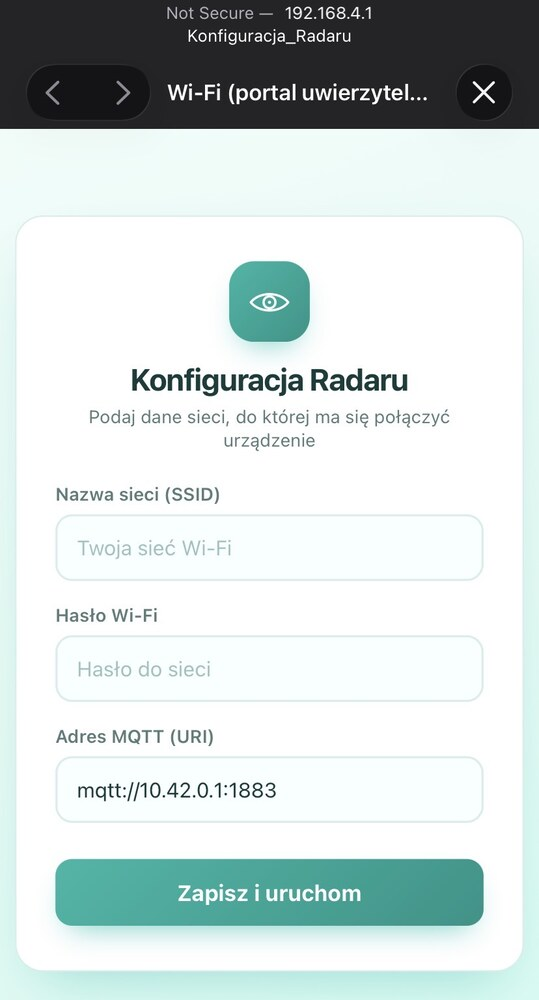
\includegraphics[width=0.23\linewidth]{captive_portal.jpg}
\caption{Portal konfiguracyjny na telefonie: SSID, has\l o Wi-Fi oraz
adres brokera MQTT (SoftAP \texttt{Konfiguracja\_Radaru}, 192.168.4.1).}
\label{fig:portal}
\end{figure}

\subsection{Publikacja MQTT i~inteligentny alarm}

W~trybie STA firmware \l \k aczy si\k e z~brokerem i~publikuje status pomieszczenia na
temacie \texttt{pokoj/101/radar} (numer pokoju jest na razie zaszyty w~kodzie).
Statyczny dashboard \l \k aczy si\k e
z~tym samym brokerem przez MQTT-over-WebSockets prosto z~przegl\k adarki i~pokazuje
karty pokoi ze statusem w~czasie rzeczywistym (rys.~\ref{fig:dash}). Prze\l \k acznik \emph{Alarm} uzbraja
doz\'or: po uzbrojeniu panel reaguje d\'zwi\k ekiem (Web~Audio, bez plik\'ow)
i~czerwonym banerem, gdy nikogo nie ma pod czujnikiem albo gdy znika \l \k aczno\'s\'c.
Kluczowe jest rozr\'o\.znienie stanu ,,pusty pok\'oj'' od ,,utrata \l \k aczno\'sci'':
watchdog wyszarza kart\k e i~oznacza j\k a jako \textsc{offline}, gdy brak danych trwa
d\l u\.zej ni\.z 10~s, \.zeby cisza czujnika nie udawa\l a spokoju.

\begin{figure}[H]
\centering
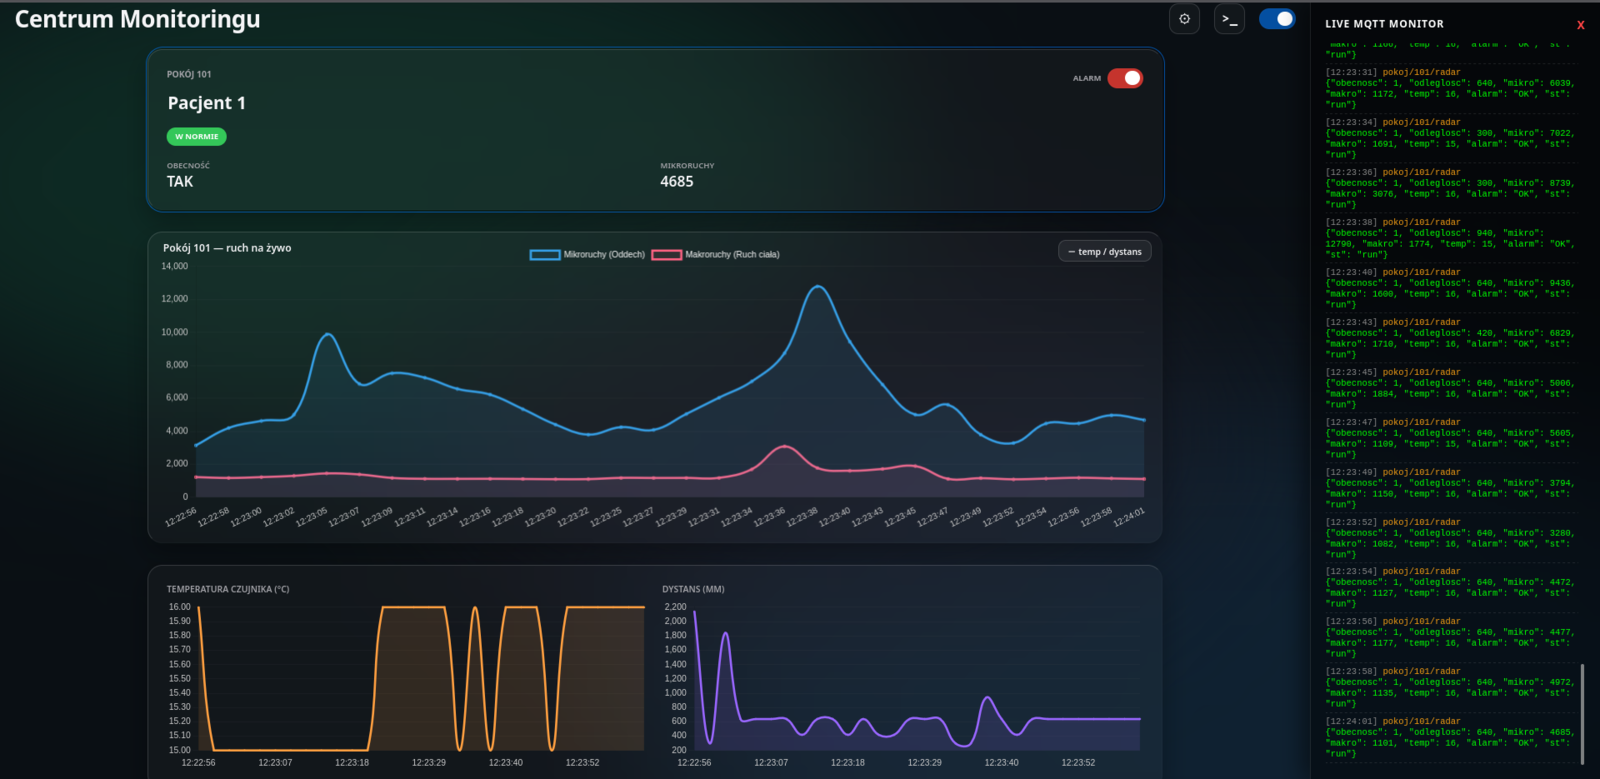
\includegraphics[width=\linewidth]{dashboard.png}
\caption{Panel opiekuna: widok pokoju z~przebiegami mikroruchu i~makroruchu,
temperatur\k a i~dystansem oraz podgl\k adem wiadomo\'sci MQTT na \.zywo.}
\label{fig:dash}
\end{figure}

\subsection{Sygnalizacja i~reset konfiguracji}

Dioda RGB sygnalizuje kolejne stany urz\k adzenia: tryb portalu
konfiguracji, \l \k aczenie z~Wi-Fi, po\l \k aczenie z~brokerem MQTT, alarm oraz b\l \k ad.
Reset konfiguracji nast\k epuje po oko\l o 3~s przytrzymania przycisku (potr\'ojny
sygna\l\ LED i~buzzera). Urz\k adzenie czy\'sci NVS i~wraca do captive portalu,
bez potrzeby ponownego wgrywania firmware. Kr\'otkie naci\'sni\k ecie przycisku
kasuje trwaj\k acy alarm d\'zwi\k ekowy.

\subsection{Instrukcja uruchomienia (quick start)}

Z~perspektywy u\.zytkownika ko\'ncowego uruchomienie sprowadza si\k e do
kilku krok\'ow, bez pod\l \k aczania do komputera:

\begin{enumerate}[leftmargin=1.6em]
  \item Zamontowa\'c czujnik pod sufitem i~pod\l \k aczy\'c zasilanie 5~V (USB).
  \item Na telefonie po\l \k aczy\'c si\k e z~otwart\k a sieci\k a
        \texttt{Konfiguracja\_Radaru}. Strona konfiguracji otworzy si\k e sama.
  \item Wpisa\'c nazw\k e i~has\l o docelowej sieci Wi-Fi oraz adres brokera MQTT
        i~zatwierdzi\'c. Urz\k adzenie zrestartuje si\k e i~zacznie publikowa\'c.
  \item Stan odczyta\'c z~diody RGB: konfiguracja / \l \k aczenie z~Wi-Fi /
        po\l \k aczenie z~brokerem / praca / alarm / b\l \k ad.
  \item W~razie potrzeby zmiany ustawie\'n przytrzyma\'c przycisk oko\l o 3~s
        (potr\'ojny sygna\l). Urz\k adzenie wr\'oci do kroku~2.
\end{enumerate}

\subsection{Bezpiecze\'nstwo}

System opiera si\k e na ci\k ag\l ej komunikacji bezprzewodowej, wi\k ec warto
wprost opisa\'c stan zabezpiecze\'n. W~obecnym prototypie przyj\k eto \'swiadome
uproszczenia: dane sieci Wi-Fi i~adres brokera s\k a zapisywane w~pami\k eci
EEPROM bez szyfrowania. Broker Mosquitto pracuje
w~trybie anonimowym, bez uwierzytelniania i~bez TLS. Ruch MQTT (1883) oraz
MQTT-over-WebSockets (9001) jest nieszyfrowany. AP konfiguracyjny jest otwarty,
a~dashboard nie wymaga logowania. Jest to akceptowalne w~izolowanej sieci
laboratoryjnej, ale nie w~docelowym wdro\.zeniu.

\subsection{Stan realizacji}

Projekt osi\k agn\k a\l\ stan dzia\l aj\k acego prototypu \emph{end-to-end}: czujnik,
firmware i~dashboard tworz\k a kompletny przep\l yw. Cztery typy detekcji
(obecno\'s\'c, upadek, przegrzanie, bezruch) dzia\l aj\k a, konfiguracja odbywa si\k e
z~telefonu przez captive portal, a~alarm wykrywa r\'ownie\.z utrat\k e \l \k aczno\'sci
z~czujnikiem.

% ===========================================================================
\section{Ograniczenia i~przypadki brzegowe}

Prototyp \'swiadomie nie by\l\ poddany pe\l nej walidacji skuteczno\'sci. Poni\.zej
zebrano znane ograniczenia metody i~bie\.z\k acej implementacji:

\begin{itemize}[leftmargin=1.4em]
  \item \textbf{Zwierz\k eta domowe.} Radar reaguje na ruch i~mikroruch, a~nie na
        sylwetk\k e. Wi\k ekszy pies lub kot w~polu widzenia mo\.ze wywo\l a\'c
        fa\l szyw\k a obecno\'s\'c. \L agodzi to monta\.z pod sufitem (zwierz\k e jest
        dalej od czujnika, s\l abszy sygna\l) oraz progi \texttt{intra}/\texttt{inter}.
  \item \textbf{Ruch firan i~przeci\k agi.} Poruszana firana przy otwartym oknie
        albo nawiew z~grzejnika czy wentylacji to drobny, powtarzalny ruch, kt\'ory
        mo\.ze podnosi\'c \texttt{intra\_score} i~da\'c fa\l szywy sygna\l\ ruchu.
        Wymaga kalibracji prog\'ow lub maskowania stref odleg\l o\'sci.
  \item \textbf{Zasi\k eg detekcji oddechu.} Mikroruch klatki piersiowej jest
        wiarygodny do oko\l o 2-3~m od czujnika. Dalej energia sygna\l u tonie
        w~szumie i~wykrywanie samego oddechu (bez wi\k ekszego ruchu) staje si\k e
        zawodne.
  \item \textbf{Jeden czujnik = jedno pomieszczenie.} Uk\l ad nie liczy os\'ob
        i~nie rozr\'o\.znia ich to\.zsamo\'sci. \'Sciany dzia\l owe t\l umi\k a
        pasmo 60~GHz, co jest zalet\k a (brak przes\l uch\'ow mi\k edzy pokojami), ale
        wymusza po jednym czujniku na pomieszczenie.
  \item \textbf{Odbicia.} Du\.ze metalowe powierzchnie i~lustra w~polu widzenia
        mog\k a dawa\'c odbicia i~zawy\.za\'c liczb\k e wykry\'c.
\end{itemize}

% ===========================================================================
\section{Podsumowanie}

Zbudowany prototyp potwierdzi\l\ trafno\'s\'c kluczowych decyzji projektowych: radar
60~GHz zapewnia detekcj\k e mikroruch\'ow bez naruszania prywatno\'sci, a~lokalna
klasyfikacja na ESP32-C6 daje reakcj\k e niezale\.zn\k a od chmury. Dalszy rozw\'oj
koncentruje si\k e na odporno\'sci \l \k aczno\'sci, dystrybucji panelu
i~bezpiecze\'nstwie (tabela~\ref{tab:roadmap}).

\begin{table}[H]
\centering
\caption{Kierunki dalszego rozwoju.}
\label{tab:roadmap}
\begin{tabularx}{\linewidth}{@{}P{0.03\linewidth} P{0.24\linewidth} L@{}}
\toprule
\textbf{\#} & \textbf{Kierunek} & \textbf{Opis}\\
\midrule
1 & Powiadomienia & Push / SMS bezpo\'srednio do opiekuna, niezale\.znie od panelu przegl\k adarkowego.\\
2 & Panel z~urz\k adzenia & Serwowanie dashboardu prosto z~ESP32 (serwer HTTP w~trybie STA), bez zewn\k etrznego brokera.\\
3 & Szyfrowanie transmisji & TLS dla MQTT (\texttt{mqtts}, port 8883) z~weryfikacj\k a certyfikatu brokera. WebSocket przez \texttt{wss}.\\
4 & Uwierzytelnianie MQTT & Login i~has\l o (lub certyfikat) per urz\k adzenie, ograniczenie temat\'ow ACL do w\l asnego pokoju.\\
5 & Ochrona danych na urz\k adzeniu & W\l \k aczenie flash encryption ESP32, aby po\'swiadczenia Wi-Fi w~NVS nie by\l y czytelne po wyj\k eciu ko\'sci.\\
6 & Zabezpieczenie konfiguracji & Has\l o WPA2 na AP konfiguracyjnym, licznik pr\'ob, logowanie do dashboardu.\\
7 & Plac\'owki i~pilota\.z & Panel wielopokojowy dla dom\'ow opieki i~szpitali oraz pilota\.z w~warunkach domowych.\\
\bottomrule
\end{tabularx}
\end{table}

Cel projektu, nieinwazyjny system detekcji obecno\'sci
i~upadk\'ow dla senior\'ow, zosta\l\ zrealizowany w~postaci dzia\l aj\k acego
prototypu. Architektura oparta na tanim ESP32-C6, jednym czujniku na pomieszczenie
i~otwartym standardzie MQTT jest \l atwa do skalowania i~integracji, co czyni
rozwi\k azanie realnym punktem wyj\'scia do wdro\.zenia produkcyjnego.

Najwa\.zniejsze wnioski z~realizacji:

\begin{itemize}[leftmargin=1.4em]
  \item \textbf{Pin \texttt{WAKE\_UP}.} Bez podci\k agni\k ecia tego pinu do 3,3~V
        radar odpowiada po I\textsuperscript{2}C samymi zerami, co \l atwo pomyli\'c
        z~b\l \k edem okablowania. By\l\ to najbardziej czasoch\l onny problem bring-upu.
  \item \textbf{Klasyfikacja na urz\k adzeniu.} Przeniesienie logiki detekcji na
        ESP32-C6 daje reakcj\k e nawet przy braku \l \k aczno\'sci z~brokerem.
  \item \textbf{MQTT-over-WebSocket.} Panel w~przegl\k adarce wymaga osobnego
        listenera WebSocket na brokerze. Bez portu 9001 dashboard si\k e nie \l \k aczy.
  \item \textbf{D\l awienie publikacji.} Ograniczenie do raz na 2~s odci\k a\.za sie\'c,
        a~natychmiastowa wysy\l ka przy alarmie zachowuje kr\'otki czas reakcji.
  \item \textbf{Captive portal.} Konfiguracja z~telefonu wyra\'znie skraca
        wdro\.zenie u\.zytkownika ko\'ncowego.
\end{itemize}

% ===========================================================================
\clearpage
\section*{Bibliografia i~\'zr\'od\l a}
\addcontentsline{toc}{section}{Bibliografia i~\'zr\'od\l a}
\sloppy

\noindent\textbf{Dokumentacja techniczna}
\begin{itemize}[leftmargin=1.4em]
  \item Waveshare A121 Range Sensor - \texttt{waveshare.com/wiki/A121\_Range\_Sensor}
  \item Acconeer Exploration Tool - \texttt{docs.acconeer.com}
  \item Datasheet ESP32-C6-WROOM-1 - \texttt{documentation.espressif.com}
  \item ESP-IDF I\textsuperscript{2}C API Reference - \texttt{docs.espressif.com/projects/esp-idf}
\end{itemize}

\medskip
\noindent\textbf{Oprogramowanie i~biblioteki}
\begin{itemize}[leftmargin=1.4em]
  \item ESP-IDF (Espressif), \'srodowisko firmware dla ESP32-C6. Wykorzystane
        komponenty: \texttt{esp\_wifi}, \texttt{mqtt\_client}, \texttt{nvs\_flash},
        \texttt{esp\_http\_server}, \texttt{driver/i2c}, \texttt{led\_strip}.\\
        \url{https://github.com/espressif/esp-idf}
  \item Eclipse Mosquitto, broker MQTT (nas\l uch na portach 1883 oraz 9001 dla
        WebSocket).\\ \url{https://mosquitto.org}
  \item MQTT.js, klient MQTT-over-WebSocket w~panelu opiekuna.\\
        \url{https://github.com/mqttjs/MQTT.js}
  \item Chart.js, wykresy przebieg\'ow mikroruchu i~makroruchu na dashboardzie.\\
        \url{https://www.chartjs.org}
\end{itemize}

\medskip
\noindent\textbf{Dane rynkowe i~statystyczne}
\begin{itemize}[leftmargin=1.4em]
  \item GUS, ,,Sytuacja os\'ob starszych w~Polsce 2024''.
  \item NCOA / CDC (USA), statystyki upadk\'ow os\'ob starszych.
\end{itemize}

\end{document}
